El siguiente ejercicio desarrollado es el análisis de las principales componentes de una imagen. Como entrada tenemos un conjunto de imágenes de caras de distintos sujetos y el número de dimeniones a las que queremos proyectar dichas imágenes.\par
La proyección en las nuevas dimensiones no es discriminativa, pero podemos utilizarla para crear clusters e identificar imágenes. 

\section{Descripción del trabajo realizado}
Una vez leídas las imágenes y cargadas en memoria como un vector de número reales, reservamos un conjunto de imágenes para el anális de las principales componentes y otro conjuto para probar cómo funciona este análisis. En este caso hemos reservado un 50\% de las imágnes para el entrenamiento y el restante 50\% para las pruebas.\par
Para cada una de las imágenes calculamos su proyección en el nuevo espacio de componentes de dimensionalidad d'. 
El caso general el algoritmo PCA, obtendría los eigenfaces (vectores propios) siguiendo el algoritmo que podemos ver en \ref{pca:general}.\par

\begin{lstlisting}[language=python,label=pca:general,caption=PCA]
        C = 1.0/n * np.dot(A,A.T)
        D,B = la.eigh(C) 
        # Ordenamos los vectores propios, primero los que más varianza recogen 
        order = np.argsort(D)[::-1] # sorting the eigenvalues
        # Ordenamos los vectores propios & los valores propios
        B = B[:,order]
        D = D[order]
\end{lstlisting}

Sin embargo en el caso de que el número de imagenes sea mucho menor que el número de dimensiones de cada imagen, realizaremos el análsis de las principales componentes siguiento el algoritmo \ref{pca:truco}.\par

\begin{lstlisting}[language=python,label=pca:truco, caption=PCA cuado n es menor d]
        if d_prime > n:
            d_prime = n
        # C: Matriz de covarianzas
        C_prime = 1.0/d * np.dot(A.T,A)
        #Delta=eigenvalues B=eigenvectors
        D_prime,B_prime = la.eigh(C_prime)

        for i in xrange(n):
            B_prime[:,i] = B_prime[:,i]/np.linalg.norm(B_prime[:,i])

        B = np.dot(A, B_prime)
        D = d/n * D_prime
        # Ordenamos los vectores propios, primero los que más varianza recogen 
        order = np.argsort(D, axis=0)[::-1] 
        # Ordenamos los vectores propios & los valores propios
        B = B[:,order]
        D = D[order]

\end{lstlisting}

Si ejecutamos PCA siguiendo este caso particular, el número máximo de dimensiones al que podremos reducir las imágenes corresponderá con el número de imágenes. Por las características de la máquina en la que hemos desarrollado esta práctica hemos empleado esta segunda implementación de PCA para tratar las imágenes. 

\subsection{Resultados}
Con el 50\% de las imágenes que habíamos reservado de cada uno de los sujetos realizaremos la fase de pruebas. Proyectaremos las imágenes en el número de dimensiones y mediante vecino más cercano etiquetaremos la imagen.\par 
Al proyectar en tan pocas dimensiones, desde 1 a 5, se pierde gran parte de la información y por eso los resultados que hemos obtenido no son los mejores.\par
En el segmento de código \ref{pca:ejec}, vemos un ejemplo de cómo ejecutar el algoritmo PCA. Recorrería todas las cara que encuentre en la ruta que le hemos especificado, utilizando el 50\% de las imágenes para entrenar y el resto para predecir una etiqueta. Los resultados de estas predicciones se guardan en un fichero de texto plano para después dibujar la gráfica con los resultados. \par

\begin{lstlisting}[language=python,label=pca:ejec, caption=Ejecución de PCA]
python pca.py -p ../data/caras/ORL -d 100 > caras100
\end{lstlisting}

Hemos desarrollado un pequeño script en python para mostrar estos resultados en una gráfica como la que podemos ver en la imagen \ref{fig:pca:resultados}.\par

\begin{figure}[h!]
  \centering
      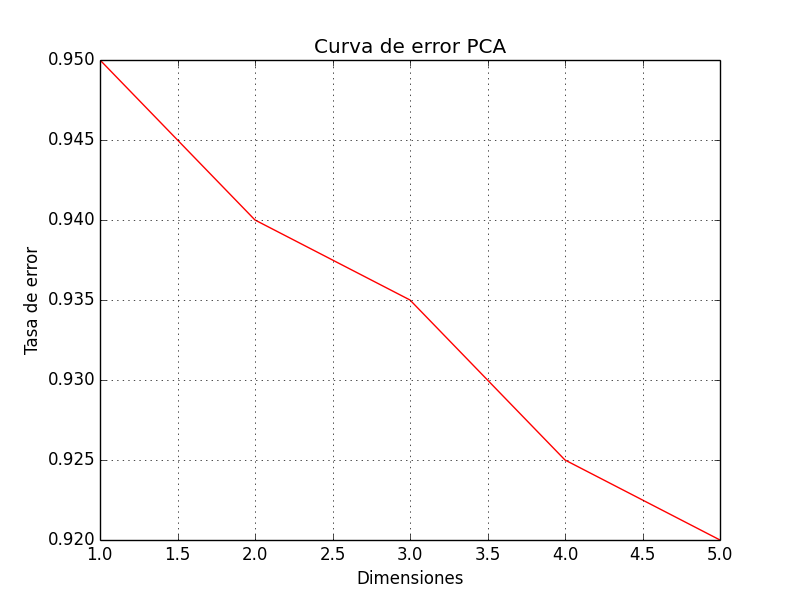
\includegraphics[width=0.5\textwidth]{../pca/outputs/salida.png}
  \caption{ Resultado PCA}
  \label{fig:pca:resultados}
\end{figure} 


